
\subsection{Đường ống dữ liệu}

Đường ống dữ liệu
bao gồm các chuỗi quy trình xử lý tự động
từ một hoặc nhiều nguồn (source) đến một đích đến (destination) để lưu trữ, phân tích hoặc phục vụ cho các ứng dụng khác.
Vì dự án này làm về miền nghiệp vụ pháp luật
nên không cần thu thập dữ liệu từ nhiều nguồn khác nhau.
Em sử dụng dữ liệu chính thống từ nhà nước là
\textbf{Văn bản pháp luật}
tại địa chỉ
\url{https://vbpl.vn}
và
dữ liệu
\textbf{Pháp Điển}
tại địa chỉ
\url{https://phapdien.moj.gov.vn/Pages/chi-tiet-bo-phap-dien.aspx}

Giao diện nguồn dữ liệu Văn bản pháp luật

\begin{figure}[H]
\centering
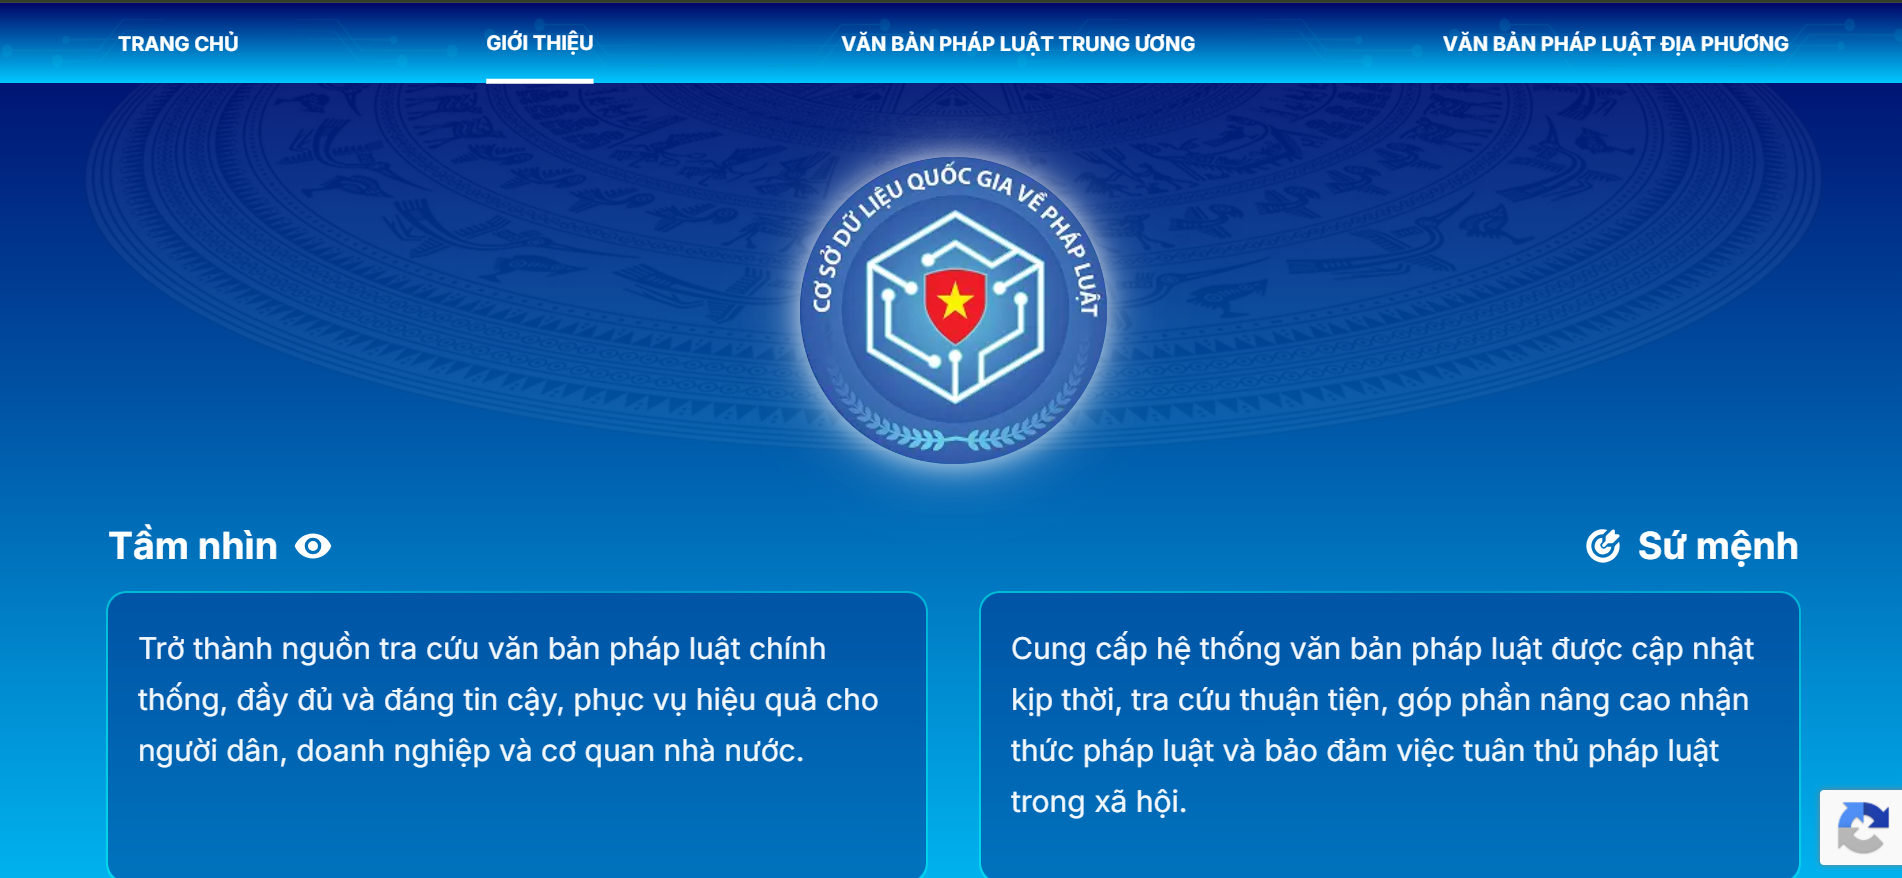
\includegraphics[width=0.95\textwidth]{pictures/Home-vbpl.png}
\caption{Giao diện nguồn dữ liệu Văn bản pháp luật}
\end{figure}

Giao diện nguồn dữ liệu Pháp Điển

\begin{figure}[H]
\centering
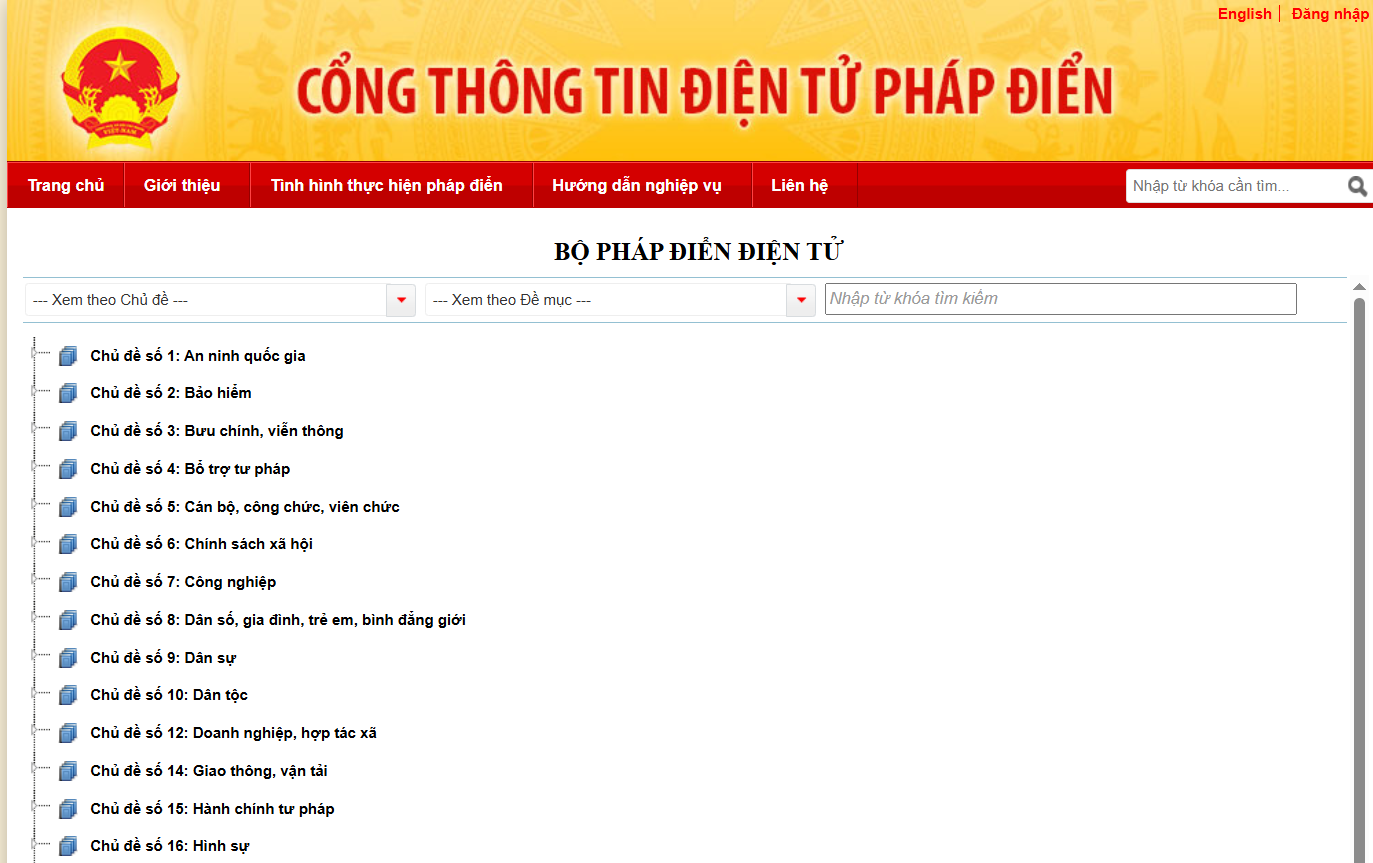
\includegraphics[width=0.95\textwidth]{pictures/Home-PhapDien.png}
\caption{Giao diện nguồn dữ liệu Pháp Điển}
\end{figure}

% Sơ đồ thu thập dữ liệu chung:

% % dùng cron-job.org để lập lịch chạy github action với trigger
% % vì github action không chạy đúng giờ như đã lập lịch thường xuyên

% % Lấy thông tin dữ liệu công việc từ database postgres

% % dùng thư viện python Scrapy để kéo thông tin dữ liệu

% % upload tải lên file kết quả đã được xử lý lên google drive để lưu trữ lâu dài

\begin{figure}[H]
\centering
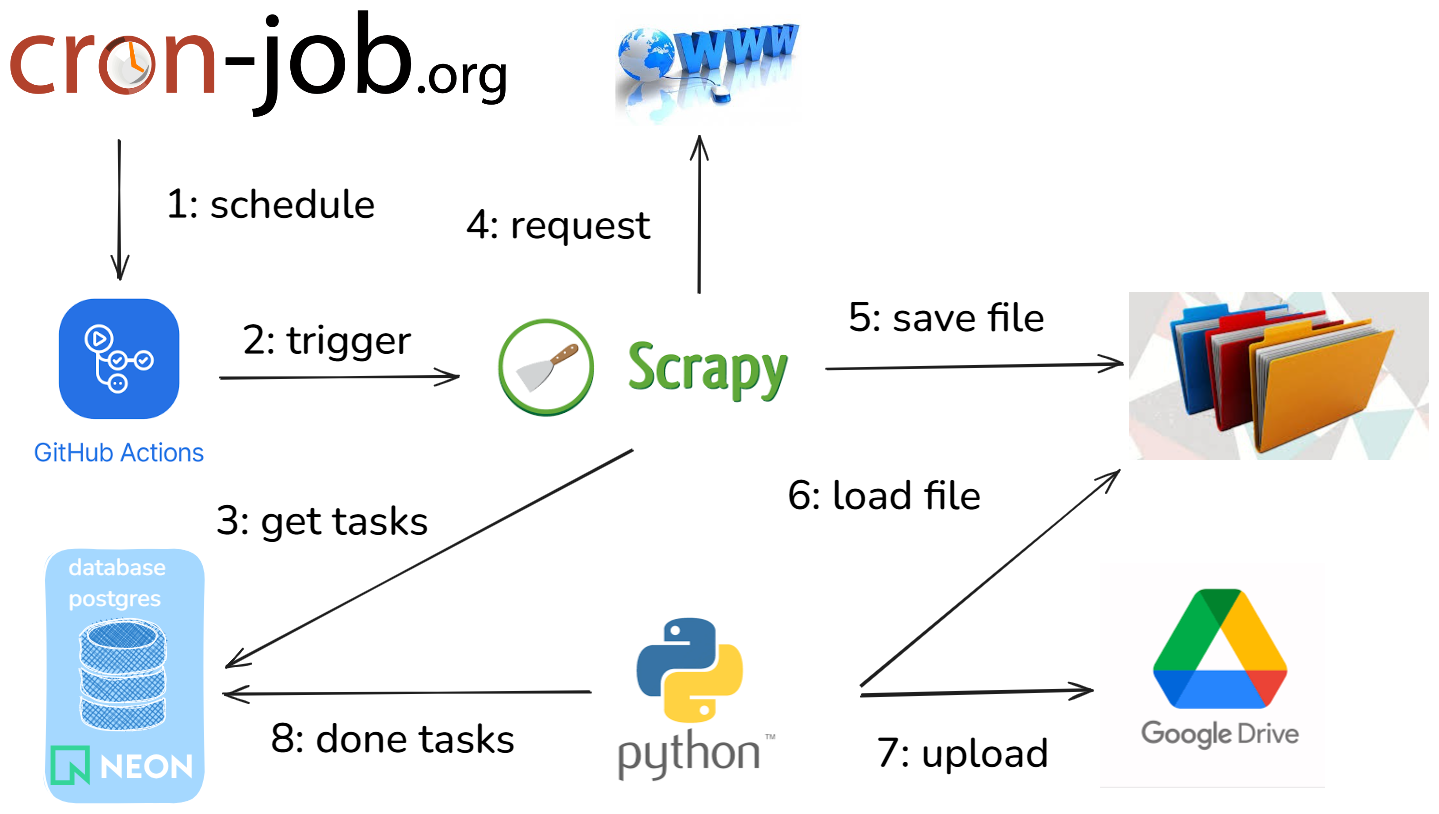
\includegraphics[width=0.95\textwidth]{pictures/crawl-data.excalidraw.png}
\caption{Sơ đồ thu thập dữ liệu chung}
\end{figure}

Tại các bước sẽ sử dụng logic so sánh hash để bỏ qua văn bản không thay đổi nội dung
giúp tiết kiệm tài nguyên và thời gian xử lý dữ liệu.

% TODO: Có so sánh hash = tiết kiệm= nhanh

\begin{figure}[H]
\centering
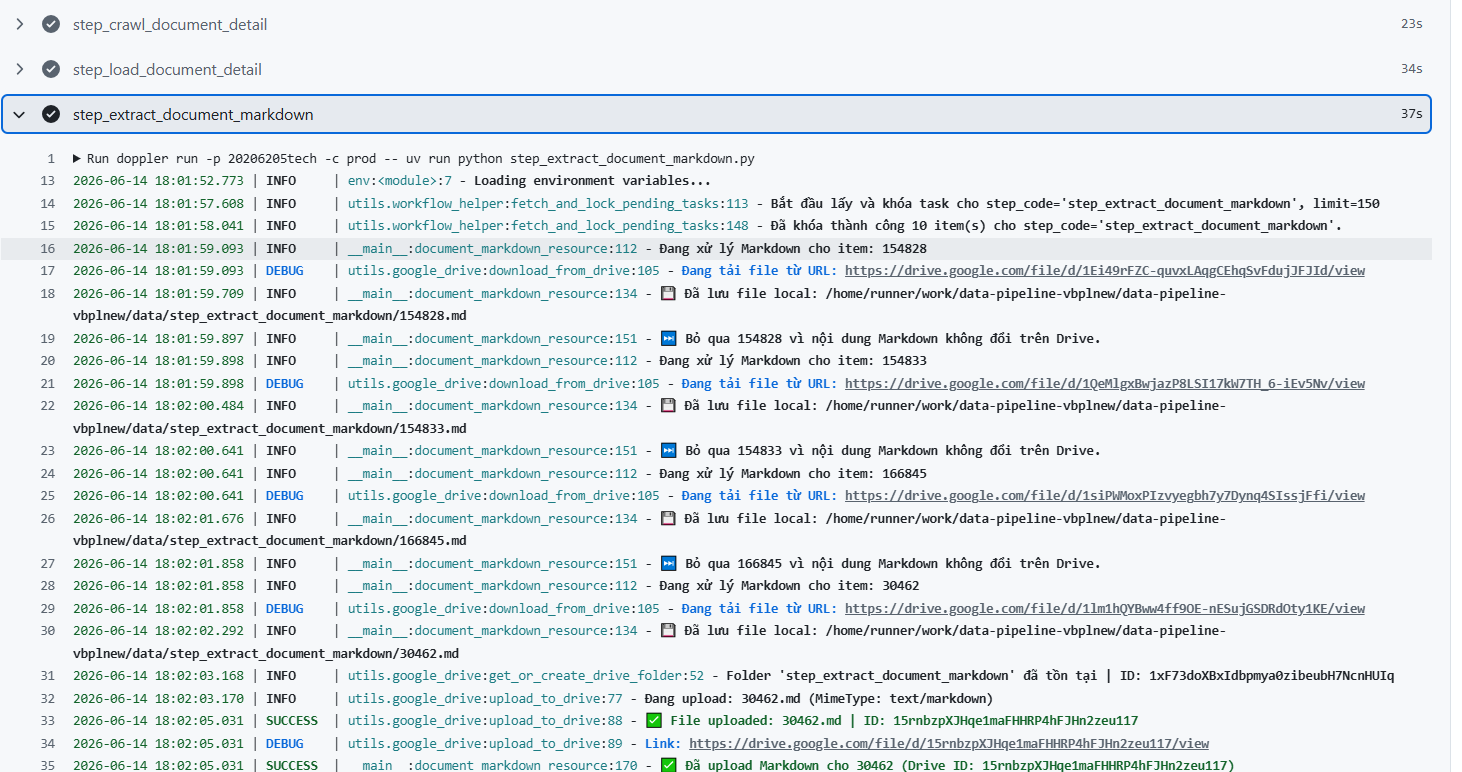
\includegraphics[width=0.95\textwidth]{pictures/data-pipeline-hash-skip.png}
\caption{Sơ đồ thu thập dữ liệu chung}
\end{figure}

Thư viện dlt (Data Load Tool)
là một thư viện Python
mã nguồn mở
giúp trích xuất dữ liệu từ nhiều nguồn khác nhau
và tải chúng vào các tập dữ liệu có cấu trúc rõ ràng.

\begin{figure}[H]
\centering
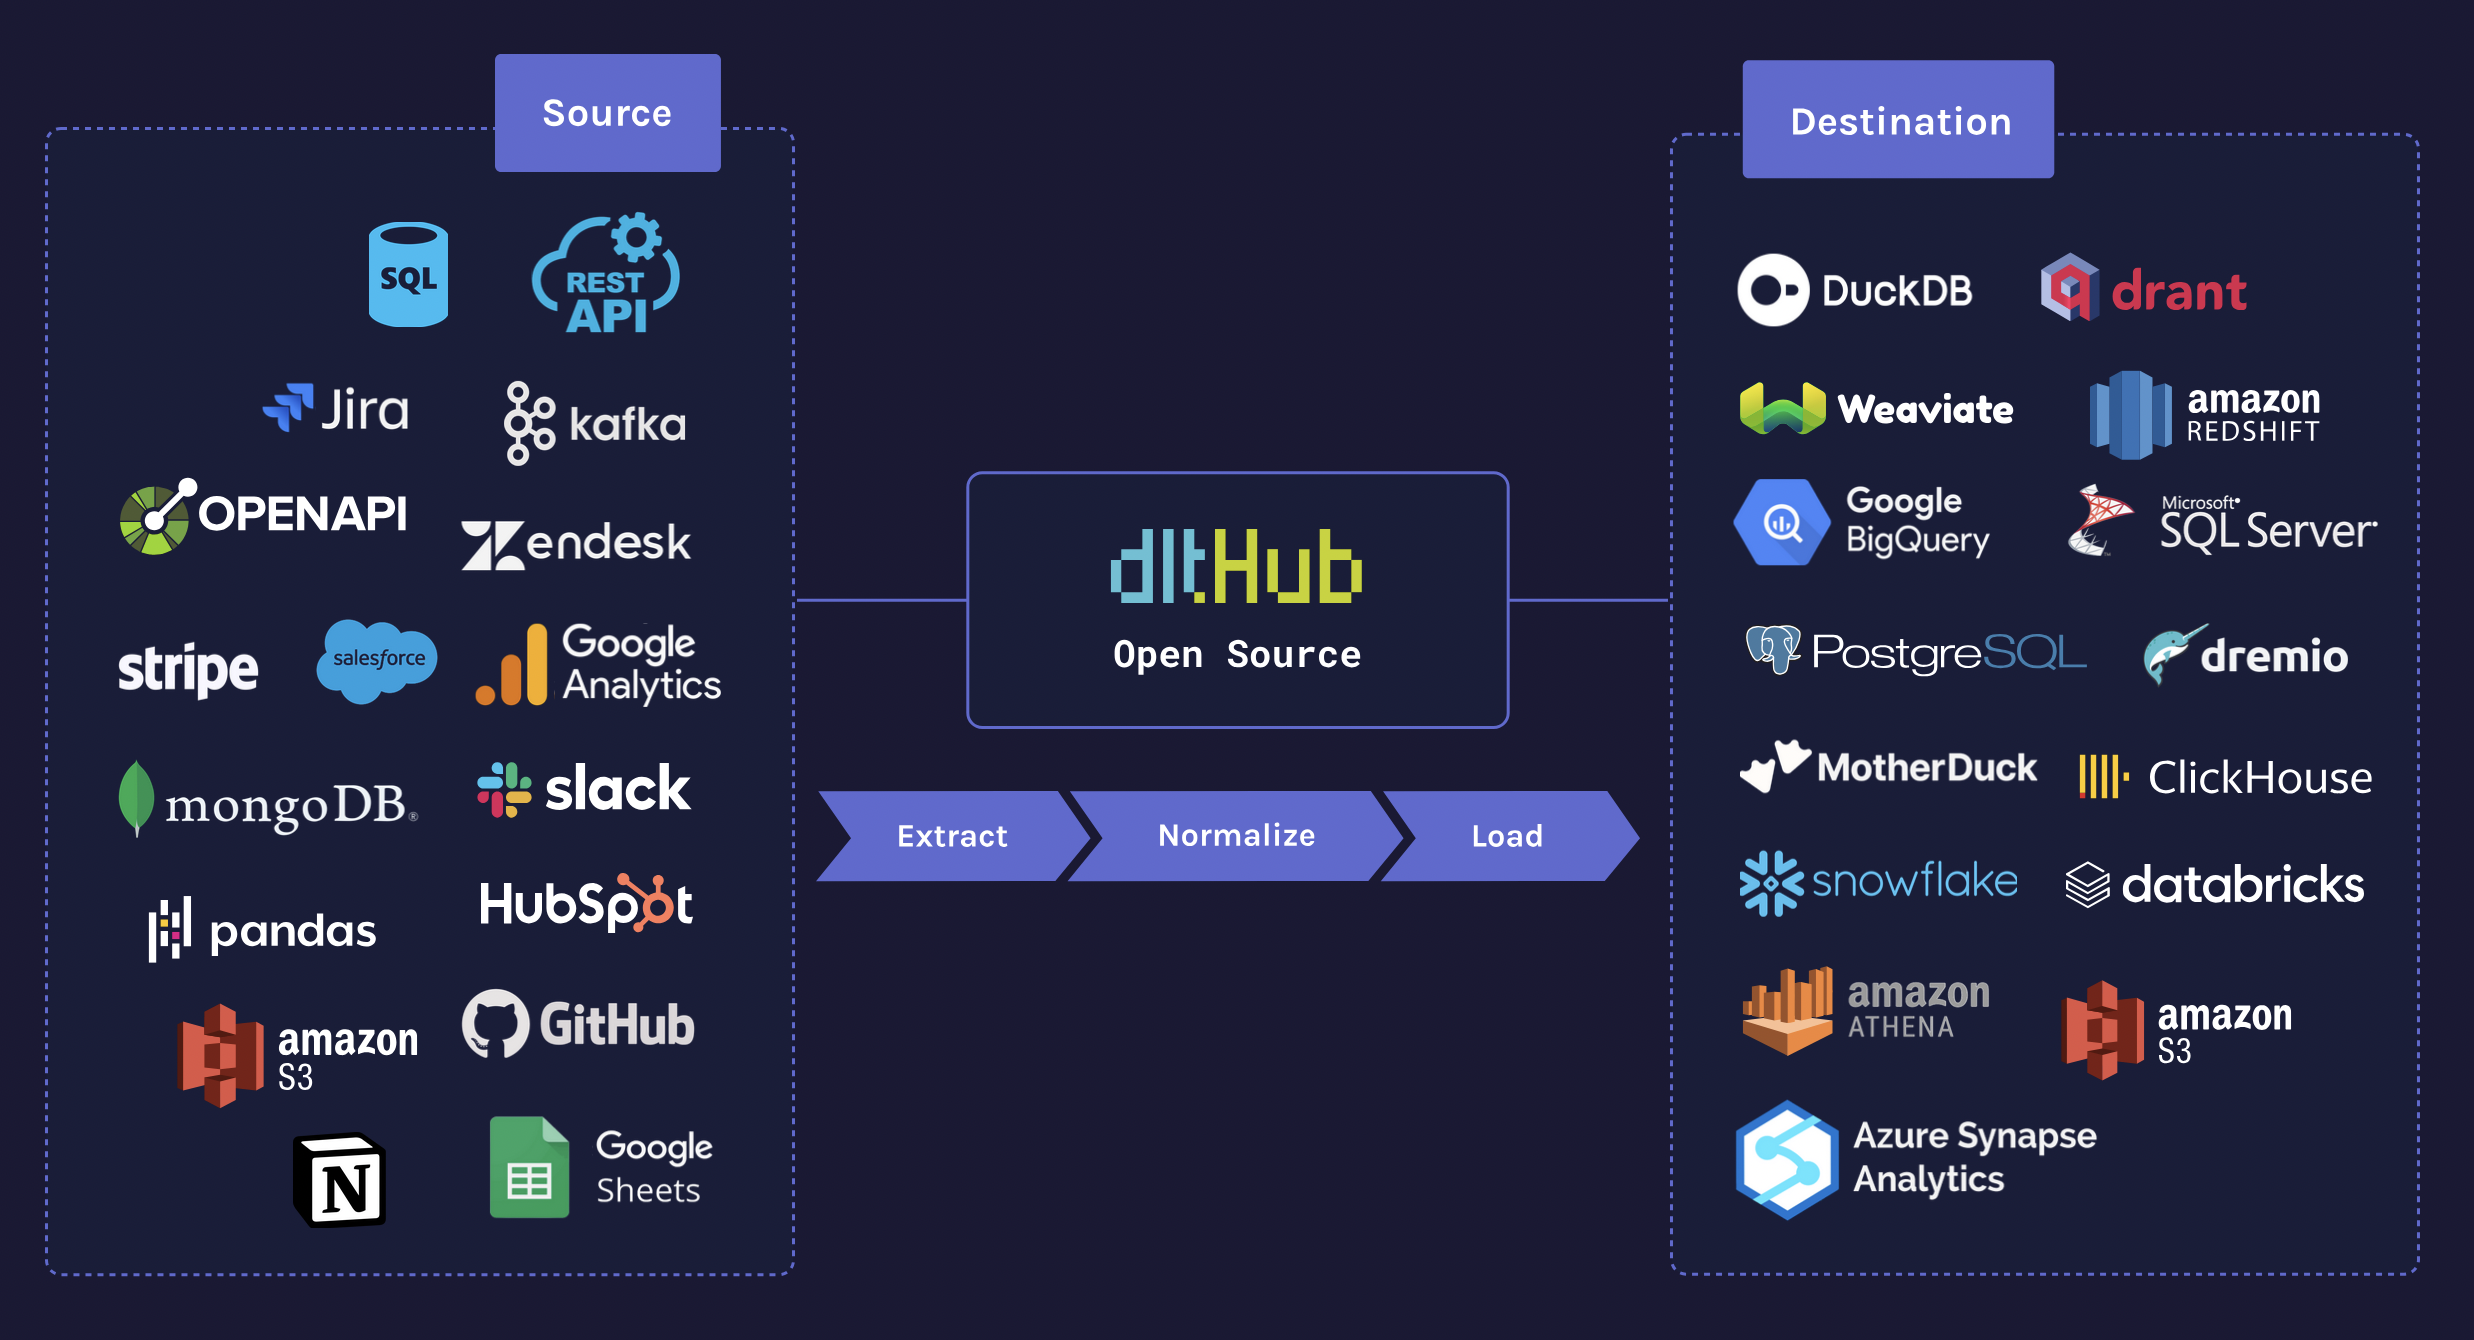
\includegraphics[width=0.95\textwidth]{pictures/dlt-onepager-c61255330e30060ca8f2fa6d7b73b600.png}
\caption{Giao diện nguồn dữ liệu Văn bản pháp luật}
\end{figure}

Việc sử dụng Data Load Tool hỗ trợ
tự động nội suy cấu trúc, kiểu dữ liệu
và xử lý mượt mà các cấu trúc dữ liệu lồng nhau
hỗ trợ tốt việc thay đổi nếu
nguồn dữ liệu có sự thay đổi

\begin{figure}[H]
\centering
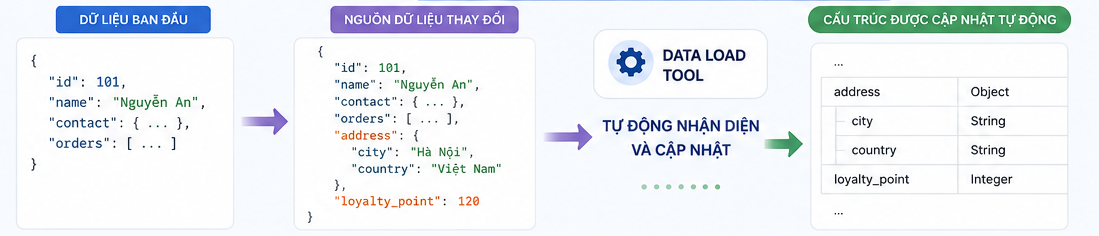
\includegraphics[width=0.95\textwidth]{pictures/dlt-auto.png}
\caption{Data Load Tool tự động thích ứng nguồn dữ liệu có sự thay đổi}
\end{figure}
